\section{Technical Implementation}
\label{section-technicalimplementation}
In this Section we outline the technical details of our implementation.

\subsection{Sentence Extractor}
\label{section-sentenceextractor}
The sentence extractor is one of the three main components and is used to extract all possible \textit{API sentences} from a given code repository. The set of API sentences that is extracted from the code repository form the \textit{sentence sample vocabulary}. That is, consider the set of all possible API sentences $S_V$ of some API vocabulary $V$. The set of extracted API sentences $\Omega$ consists of a sample of observations that is a subset of the superset of the API vocabulary $\Omega \subseteq S_V$.
We use this sample set to train API-specific $n$-gram language models.

Within a given namespace or \textit{API}, we refer to possible code expressions on the API as \textit{API tokens}.
An API token is an \textit{invocation expression} and may comprise one of three different types of invocations:

\begin{enumerate}
	\item \textbf{Instance operation}
	
	Any 'normal`, non-static operation on an instance of some class other than its constructor.
	
	\item \textbf{Static operation}
	
	Any static operation on an instance of some class.

	\item \textbf{Class constructor}
	
	Constructor called upon object instantiation.
\end{enumerate}

We used the static repository data from the KaVE project \cite{Kave} and extracted API sentences from all contexts within this data set.

\subsubsection{API Token}
\label{section-apitoken}

In order to work with the data that we extract from the static repository data and to be able to build API sentences using tokens we introduce a class \textit{APIToken}.
An APIToken is a single invocation expression that includes a namespace, type, invocation and operation.

The class APIToken extends the class MethodName and is thus naturally suited to work with and represent the data from \cite{Kave}. Other than shorthand methods and minor adjustments to existing methods, the APIToken class does not differ much from MethodName.

\subsubsection{API Visitor}
\label{section-apivisitor}

The static repository data from the KaVE project contains several preprocessed code repositories represented as \textit{Simplified Syntax Trees} (SSTs) \cite{Kave}.

An SST can comfortably be traversed and processed using the Visitor pattern. Particularly, the KaVE project \cite{Kave} already provides several interfaces and classes that allow for a straightforward implementation of a visitor to extract API sentences from a given SST.

We introduce a class \textit{APIVisitor} which implements the interface ISSTNodeVisitor to process SSTs.

In each visit method, the APIVisitor is given an ISSTNode statement or any extension or implementation of an ISSTNode statement and an \textit{APISentenceTree} context such that the statement or expression is added to the context if it is an invocation expression. Recall that we are only interested in invocations and hence not extract any other expressions. The APIVisitor will add every invocation expression to the context and ignore all other expressions.

Additionally, an SST may include statements that would allow for several different API sentences. We call such statements \textit{branching statements}. A branching statement is an if-else-expression or any other conditional statement that would allow for multiple different execution paths and thus multiple different API sentences. We collect the tokens at which branching statements appear in the context so that in a later step we can compute multiple sentences from a single context. The details of how this is done is outlined in the following Section.

An SST context may include multiple methods. We process SSTs on a per-method basis and create a single APISentenceTree per such method.

\subsubsection{API Sentence Tree}
\label{section-apisentencetree}

We introduce the class \textit{APISentenceTree} and use it as our context in the APIVisitor. That is, an APISentenceTree will store a tree representation of all relevant APITokens from an SST that was processed by the APIVisitor.

Particularly, an APISentenceTree includes a list of APITokens and a map with lists of APISentenceTrees as entries and APITokens as keys. This map stores the branches.
Whenever the APIVisitor encounters a branching statement, it will create a new branch in the APISentenceTree with the \textit{last valid token}. The last valid token is the last token that was added to the APISentenceTree or an empty 'null-token` used as a placeholder if there was no token added previously.

Using a token for branching means that a new entry is added to the map for this token.
The entry is a list of APISentenceTrees and is empty at first, meaning, that it does not contain any tokens.
A single token can be used to branch multiple times. Suppose an if-else-statement with both, an if-block as well as an else-block. In this case, the last valid token will be used to create two branches, one for the if-block and one for the else-block.
Similarly, in switch statements a single token might be used for branching several times. For branching statements in iterations, we only branch once.

In a later step, after the SST was processed by the APIVisitor, a list of all possible API sentences can be computed from the APISentenceTree. We call this process \textit{flatten}.

\begin{figure}[H]
	\centering
	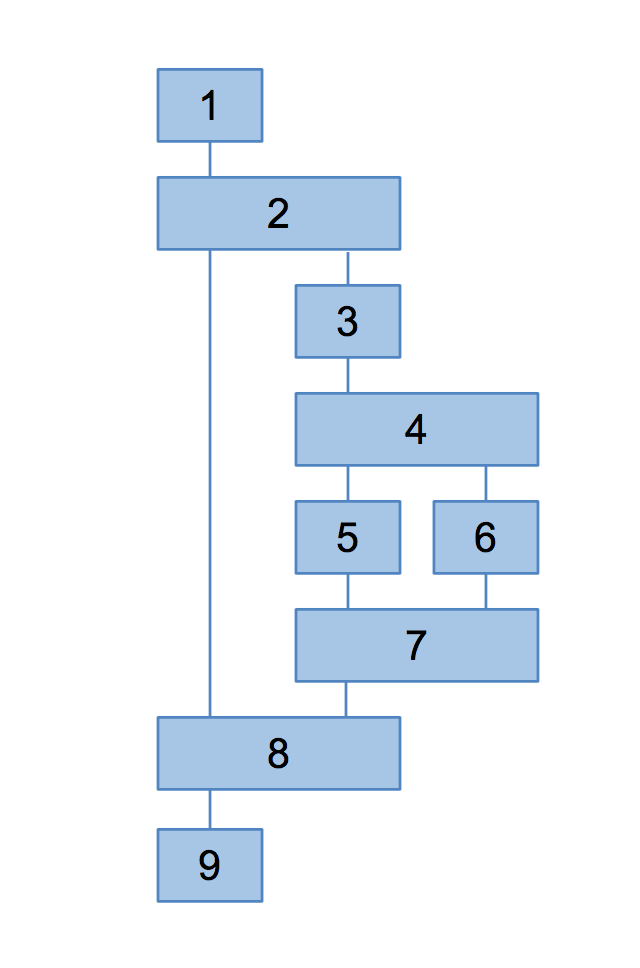
\includegraphics[width=2in]{./section-chapter2/images/apisentencetree-ex1.png}}
	\caption{SST to APISentenceTree Example}
	\label{fig:asp-1}
\end{figure}

Consider the (even more simplified) SST in Figure \ref{fig:asp-1}. Suppose that every wider box represents a branching statement and the boxes underneath until the next wider box represent boxes in these branches such that all connected boxes belong to the same branch.
There are two branching tokens, namely token $2$ and token $4$. Token $2$ will only cause a single additional branch whereas token $4$ will be used for two branches.
The APISentenceTree will have the following structure:

\begin{center}
	\mbox{$1 \rightarrow 2 \rightarrow 8 \rightarrow 9$}\\
	\mbox{$2: [3 \rightarrow 4 \rightarrow 7]$}\\
	\mbox{$4: [5]$}\\
	\mbox{$4: [6]$}
\end{center}

From this, we will be able to flatten the APISentenceTree to obtain the following sentences:

\begin{center}
	\mbox{$[1,2,8,9]$}\\
	\mbox{$[1,2,3,4,5,7,8,9]$}\\
	\mbox{$[1,2,3,4,6,7,8,9]$}
\end{center}

Furthermore, as we are interested in obtaining an $n$-gram language model on a per-API-basis, we \textit{bucketize} API sentences after obtaining them from the flattened APISentenceTrees. In this process, we create new API sentences from those that we extracted such that all API tokens in a single API sentence belong to the same namespace. See Figure \ref{fig:bucketize-ex1} for an example on bucketizing. Notice that the second API sentence (left in the figure) contains API tokens with different namespaces. They will be split into API sentences for each namespace and then stored accordingly.

This is in accordance with the original paper \cite{Santos2017stepwise}\footnote{For future work, it would be very interesting to train $n$-gram language models using the API sentences as they were extracted, i.e. non-bucketized, as we believe that this approach might allow for useful recommendations across multiple APIs.}


\begin{figure}
	\centering
	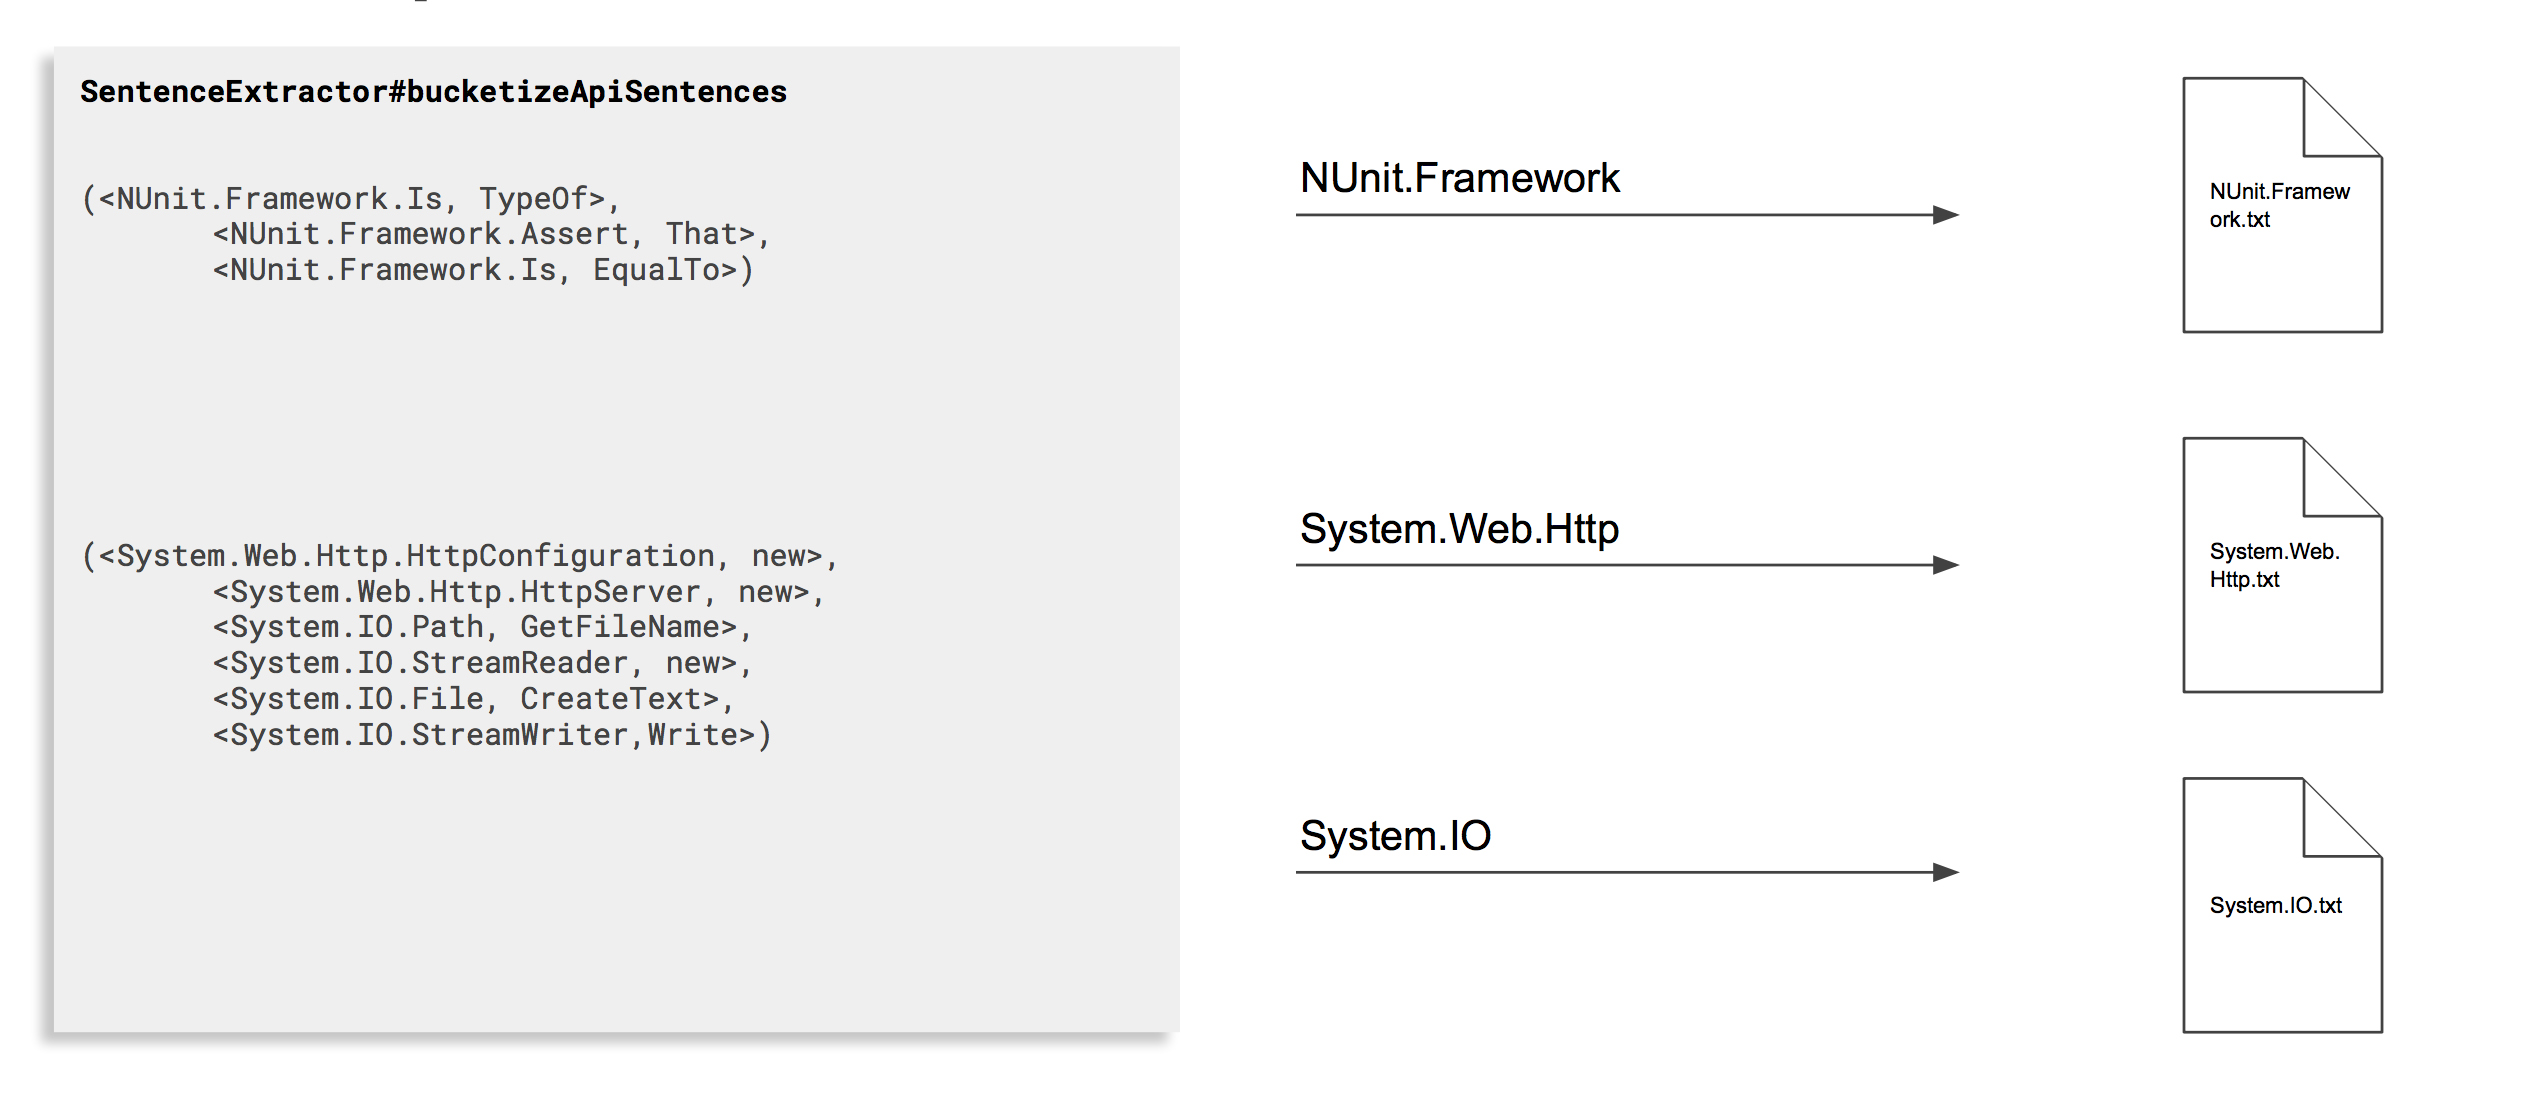
\includegraphics[width=2in]{./section-chapter2/images/bucketize.jpg}
	\caption{Bucketize Example}
	\label{fig:bucketize-ex1}
\end{figure}




\subsection{Recommender}
